\documentclass[aspectratio=169]{beamer}
\usetheme{Madrid}
\usecolortheme{seahorse}
\usepackage{booktabs}
\usepackage{xcolor}

\title[AEIC on ImageNet-1k]{Ultra-Low Bitrate Perceptual Image Compression\\with Shallow Encoder (AEIC) on ImageNet-1k}
\author{Benjamin Had\v{z}ihasanovi\'{c} \and Tarik \v{C}aluk}
\institute{Multimedia Systems — project (paper: Zhang, Liu, Chen, CVPR 2026)}
\date{\today}

\begin{document}

% ---------- Slide 1 ----------
\begin{frame}
  \titlepage
  \centering\footnotesize
  Paper: arXiv:2512.12229 \quad Code: github.com/LuizScarlet/AEIC
\end{frame}

% ---------- Slide 2 ----------
\begin{frame}{The problem}
  \begin{itemize}
    \item Ultra-low bitrate compression: $<0.05$ bits per pixel — for satellite/IoT/edge uplinks.
    \item Classic codecs collapse here (blur, blocking); \emph{generative} codecs synthesize
          plausible detail at the decoder.
    \item But existing generative codecs put \textbf{huge pretrained encoders} (VAE/tokenizers)
          on the \emph{sender} — exactly the weak device!
    \item Paper's question: \textbf{how shallow can the encoder be at ultra-low bitrates?}\\
          Insight: less rate $\Rightarrow$ less information to extract $\Rightarrow$ much simpler encoder suffices.
  \end{itemize}
\end{frame}

% ---------- Slide 3 ----------
\begin{frame}{The AEIC algorithm — architecture, training, distillation}
  \begin{enumerate}
    \item \textbf{Shallow encoder} $g_a$: tiny StarNet CNN, image $\to$ latent ($32\times$ downsampling).\\
          AEIC-ME: 3.09M params / 204 KMACs/px \quad AEIC-SE: \textbf{0.94M / 46 KMACs/px, 35.8 FPS @1080p}
    \item \textbf{Entropy model}: scale--mean hyperprior + quadtree spatial context;\\
          Gaussian-mean rounding + rANS arithmetic coding.
    \item \textbf{One-step diffusion decoder}: latent $\to$ SD-Turbo latent space $\to$
          LoRA-adapted UNet, \emph{single} denoising step (+ structural residual) $\to$ pruned VAE
          decoder. All generative ``heavy lifting'' happens at the receiver.
  \end{enumerate}
  \medskip
  \textbf{Training}: relaxed-rate pretraining (MSE+LPIPS) $\to$ ultra-low-rate GAN fine-tune
  (DINOv3 discriminator, DISTS) $\to$ high-res fine-tune.\\
  \textbf{Dual-side distillation} ME $\to$ SE (encoder latents + decoder/UNet features) shrinks
  the shallow encoder's quality gap to $<3\%$. Released: 5 rate points (\texttt{ft2}--\texttt{ft32}).
\end{frame}

% ---------- Slide 5 ----------
\begin{frame}{Our implementation (Google Colab, T4 GPU)}
  \begin{itemize}
    \item Official repo + released AEIC-SE checkpoints; no retraining.
    \item \textbf{Data}: ImageNet-1k validation, streamed from Hugging Face;
          first 500 images with short side $\geq 256$ px, exported losslessly as PNG.
    \item \textbf{5 small code changes}:
      \begin{enumerate}
        \item C++ rANS engine made optional (bpp from entropy-model likelihoods; verified vs.\ real bitstreams),
        \item xformers $\to$ PyTorch SDPA attention,
        \item \texttt{torch.compile} off (ImageNet sizes vary $\Rightarrow$ constant recompilation),
        \item local port of \texttt{update\_patch\_fid} (FID/256) — \texttt{neuralcompression} no longer builds,
        \item KID subset size $1000 \to 50$ (small images = few 256px patches).
      \end{enumerate}
    \item Pinned \texttt{diffusers==0.25.1}, \texttt{transformers==4.46.3}, \texttt{peft==0.13.2};
          kept Colab's PyTorch.
  \end{itemize}
\end{frame}

% ---------- Slide 6 ----------
\begin{frame}{Metrics (same as the paper)}
  \begin{itemize}
    \item \textbf{bpp} — rate: compressed bits / pixels.
    \item \textbf{PSNR, MS-SSIM} $\uparrow$ — pixel/structural fidelity (``distortion'').
    \item \textbf{LPIPS, DISTS} $\downarrow$ — deep-feature perceptual similarity to the original.
    \item \textbf{FID, KID} $\downarrow$ — distance between Inception feature \emph{distributions}
          (patch-wise, MS-ILLM protocol) — realism without pixel alignment.
  \end{itemize}
  \medskip
  Together: the \textbf{rate--distortion--perception} trade-off. Generative codecs willingly
  trade PSNR for LPIPS/DISTS/FID at these rates.
\end{frame}

% ---------- Slide 7 ----------
\begin{frame}{Problems faced \& solutions}
  \begin{itemize}
    \item \textbf{Dependency conflicts} (repo pins torch 2.1 + old diffusers; \texttt{neuralcompression}
          fails to build) $\to$ pin only API-critical libs, keep Colab PyTorch, inline the one
          function used from \texttt{neuralcompression}.
    \item \textbf{Gated ImageNet} $\to$ HF token + streaming (no 6.7 GB download); ungated mirror as fallback.
    \item \textbf{C++ entropy coder build} (fetched pybind11 v2.10.4 predates Python 3.12) $\to$
          one-line guard for the main pipeline; bumped pybind11 to v2.13.6 for the verification
          build: real 0.0180 vs.\ estimated 0.0167 bpp ($\approx$7\% header/rANS overhead).
    \item \textbf{Variable image sizes} $\to$ disable torch.compile; filter $<256$ px (MS-SSIM constraint).
    \item \textbf{Colab session limits} $\to$ per-checkpoint logs/outputs; resumable runs.
  \end{itemize}
\end{frame}

% ---------- Slide 8 ----------
\begin{frame}{Results on ImageNet-1k val (500 images)}
  \centering
  {\footnotesize
  \begin{tabular}{lccccccc}
    \toprule
    ckpt & bpp & PSNR & MS-SSIM & LPIPS & DISTS & FID & KID\\
    \midrule
    ft32 & 0.0049 & 17.71 & 0.576 & 0.374 & 0.202 & 60.1 & 0.0064\\
    ft8  & 0.0167 & 19.99 & 0.728 & 0.237 & 0.144 & 39.6 & 0.0015\\
    ft2  & 0.0431 & 21.75 & 0.825 & 0.157 & 0.106 & 26.5 & $-0.0002$\\
    \midrule
    JPEG$_{q=1}$ & 0.1915 & 21.07 & 0.809 & 0.547 & 0.411 & 151.5 & 0.0651\\
    \bottomrule
  \end{tabular}}
  \smallskip

  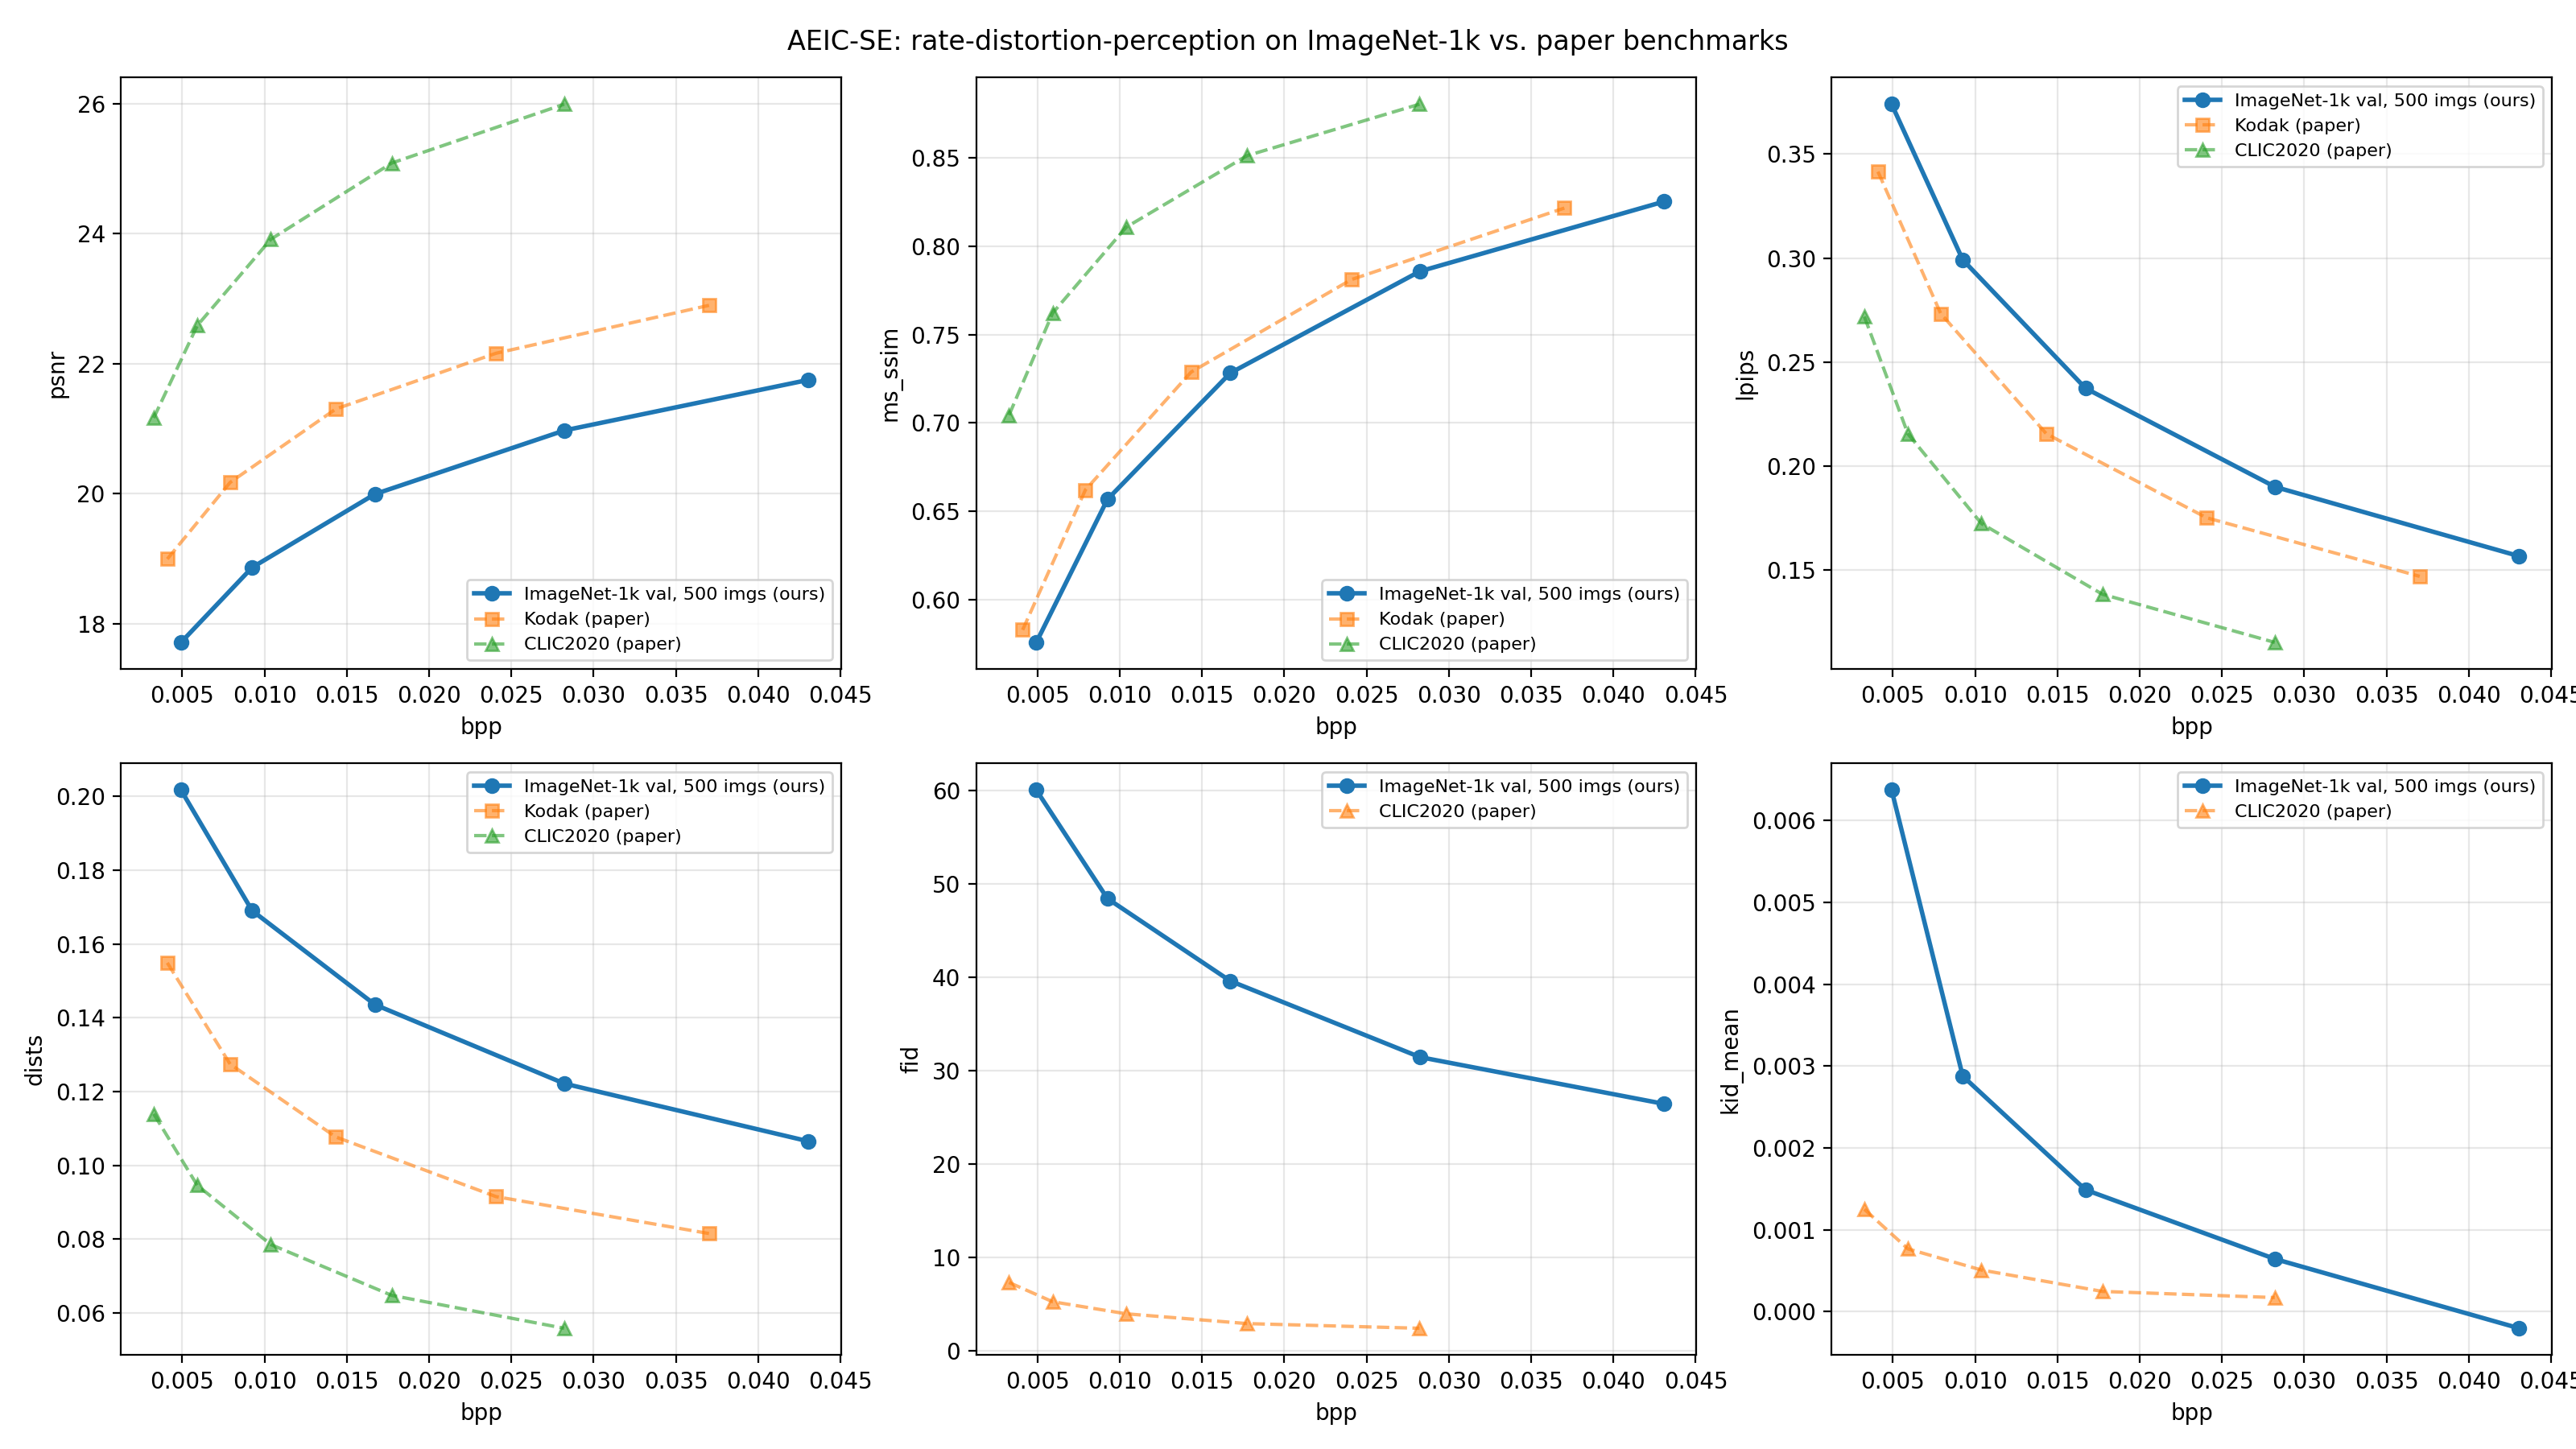
\includegraphics[width=.62\linewidth]{rd_curves_imagenet.png}

  \tiny full 5-point table in the report
\end{frame}

% ---------- Slide 9 ----------
\begin{frame}{One image across the full rate sweep}
  \centering
  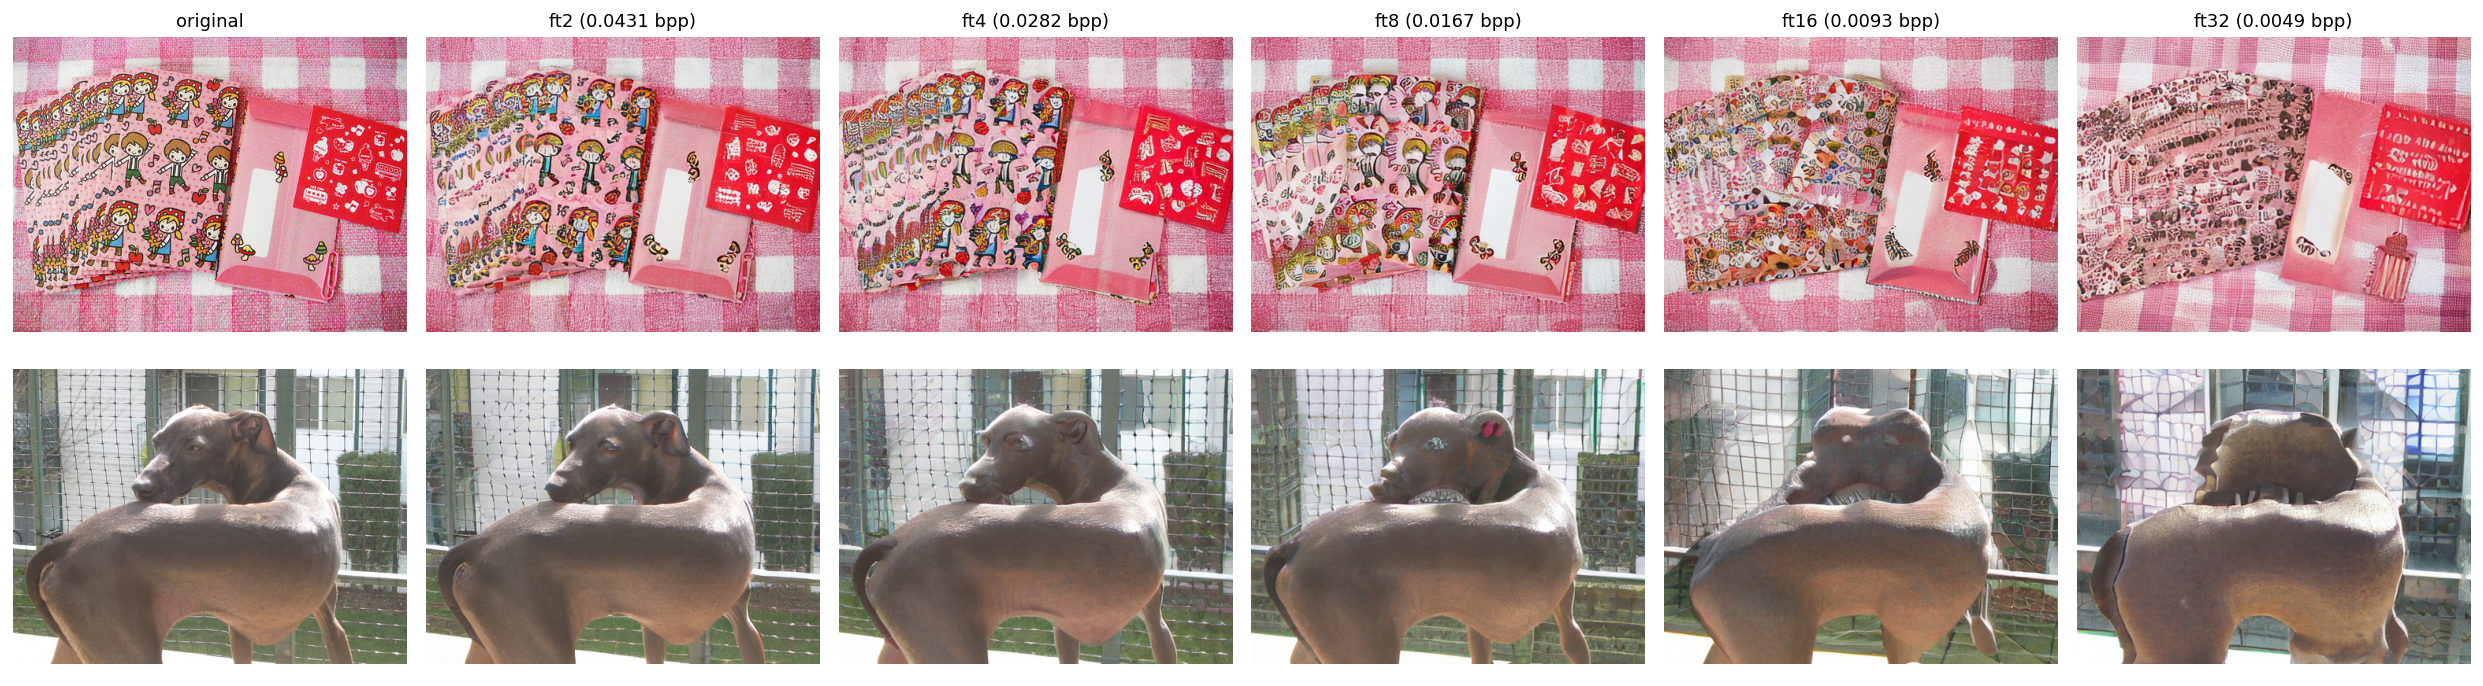
\includegraphics[width=\linewidth]{rate_sweep_imagenet.png}
  \begin{itemize}
    \item Degradation is gradual and content-dependent: printed text and fine patterns (top) are
          re-synthesized ever more loosely; the fur and thin wire fence (bottom) are visibly
          redrawn only at the lowest rate.
    \item Subjectively: down to ft16 (0.009 bpp) hard to distinguish from the original at normal
          viewing distance; at ft32 (0.005 bpp), differences are visible at any distance.
  \end{itemize}
\end{frame}

% ---------- Slide 10 ----------
\begin{frame}{Interpretation}
  \begin{itemize}
    \item All 7 metrics improve monotonically with rate (0.0049 $\to$ 0.0431 bpp) — same
          trade-off shape as the paper's curves: \textbf{the codec generalizes} to unseen data.
    \item bpp $\approx$ 50\% higher than CLIC at the same checkpoint (0.0049 vs.\ 0.0033):
          small images ($\sim$0.2 MP) amortize the fixed hyper-latent + padding overhead poorly.
    \item MS-SSIM almost identical to Kodak (0.576–0.825 vs.\ 0.583–0.822), PSNR $\sim$1 dB lower:
          at $<0.05$ bpp the codec \emph{hallucinates} texture rather than preserving pixels
          (and ImageNet ``originals'' are JPEGs themselves).
    \item FID 26.5–60.1 $\gg$ CLIC's 2.5–7.4 — only $\sim$600 patches vs.\ $\sim$20k (FID is biased
          upward at small sample sizes); the \emph{trend} is the signal. KID at 0.043 bpp is
          $\approx 0$ (even slightly negative): reconstructions statistically indistinguishable.
    \item \textbf{JPEG can't reach this regime}: its floor is 0.19 bpp ($4.4\times$ ft2) with
          similar PSNR but LPIPS 0.55 vs.\ 0.16 and FID 151 vs.\ 26 — PSNR alone misleads.
  \end{itemize}
\end{frame}

% ---------- Slide 10 ----------
\begin{frame}{Possible improvements \& conclusion}
  \textbf{Improvements}
  \begin{itemize}
    \item Resolution-adaptive overhead (hyper-latent/padding) for small images.
    \item One variable-rate model instead of 5 checkpoints (rate conditioning).
    \item Distill the one-step UNet $\to$ lightweight \emph{decoding} too; semantic bit allocation
          (faces/text); video extension.
  \end{itemize}
  \medskip
  \textbf{Conclusion}: AEIC runs on ImageNet-1k with only 3 minor code changes and keeps its
  rate--distortion--perception behaviour on unseen data — supporting the claim that at ultra-low
  bitrates a 0.94M-parameter encoder is enough when paired with a one-step diffusion decoder.
\end{frame}

\end{document}
